% vim:ts=4:sw=4
% Copyright (c) 2014 Casper Ti. Vector
% Public domain.

\chapter{实验和展望}
\section{系统测试}
为了分析和评估本论文提出的基于人脸识别的匹配算法的有效性和可用性,我们使用了该算法编写的基于婚恋数据的匹配好友的应用进行了实验测试。本实验主要基于不同算法的匹配系统进行了分析评估。

本实验对于两个方面进行了分析和评估:
\begin{enumerate}
\item 数据库用户分析
\item 测试用户对于不同匹配算法的满意度
\end{enumerate}

\subsection{数据库用户分析}
由于数据库的特性,对于数据库的用户进行分析是非常具有必要性的,具有相同属性的人成为好友的概率往往会非常的高。但由于本文的数据库的内容的一些缺失性,在世纪佳缘上的很多信息都不是必须填写的信息,所以本文只对于数据库的年龄属性这一必要的属性进行了分析。

通过数据库的采取的3000条数据进行分析,对于数据库的用户数据进行了统计。测试用户和数据库的用户的年龄分布如下图
\begin{figure}[h] 
\begin{minipage}[t]{\linewidth}

\centering

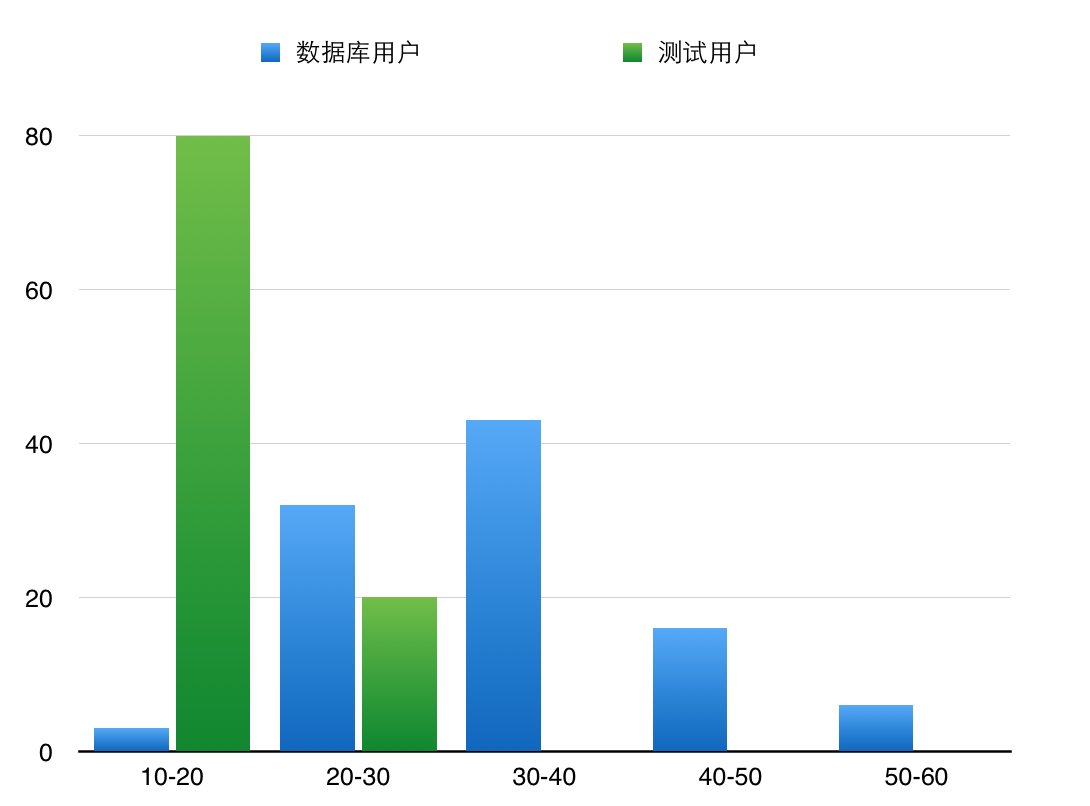
\includegraphics[width=\textwidth]{img/chap5/exp1.png}
\caption{年龄分布\label{instagram}}
\end{minipage}
\end{figure}

通过图5.1,我们可以看出在数据库中的用户的年龄都偏大,超过半数的用户都超过了30岁,而测试用户却相反的半数以上都为30岁以下的青年人。带来这种差异的原因主要是数据库数据来源的特性,由于是婚恋网站,所以大多数的用户年龄都偏大,以及本文所邀请的用户的局限性主要限定在大学周围。

由于年龄段的不同,用户有着不同的兴趣和审美观,而年龄差异过大的也并不适合成为一个社交圈子里的人。这种差异给匹配算法带来了一些不确定性。


\subsection{匹配算法实验}
\subsubsection{实验设计}
本文对于匹配算法的评判的标准为用户给出对于匹配结果的满意程度,这里的满意程度鉴于用户密度和数据粒度的关系,设成了1~10十个不同的分数。

评选的方式为用户提交自己的照片,通过10张对于用户照片给出的匹配结果,用户统计一下自己对于这10个结果的满意程度,从而对于一个匹配算法给出一个最终的满意程度。
\subsubsection{实验结果}
总共20人参加了该实验的测试,该实验的满意度的分数为10级,如设计所述,测试用户对于一个匹配测试算法给出的10个推荐好友进行评分,作为最终的检测结果。而对于不同的匹配算法的满意度的结果如图5.2所示。
\begin{figure}[h]
\begin{minipage}[t]{1\linewidth} 
\centering
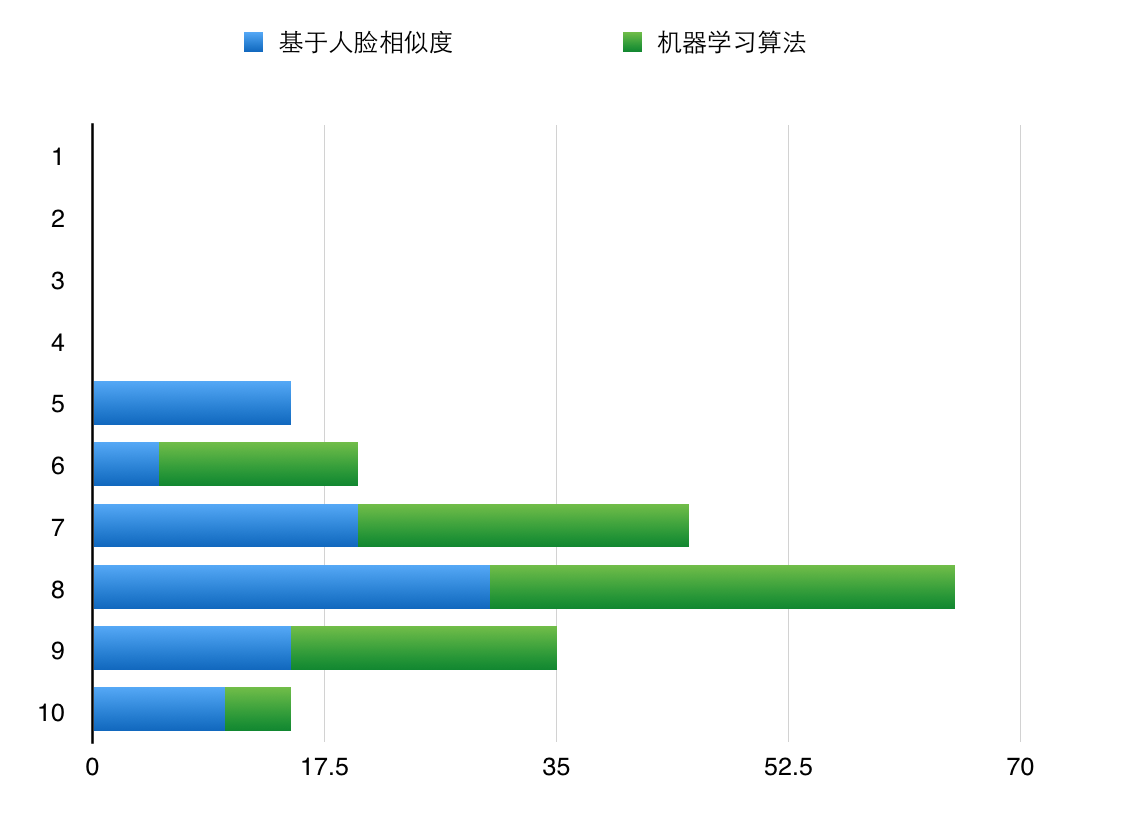
\includegraphics[width=\textwidth]{img/chap5/exp2.png}
\caption{满意度统计结果\label{instagram}}
\end{minipage}
\end{figure}
从表中可以看出由于加入了更多的特征到了匹配算法中,机器学习算法的用户的满意度对于原有的匹配算法的效果有了一定的提升,而原有的匹配的满意程度也不低,说明了经过人脸识别技术的好友匹配算法有了一个比较好的效果。但由于个人主观的问题,还需要进一步时间去检验该不同匹配算法的优劣。但从整体结果来看,还是比较可喜的。
\section{展望}
\begin{figure}[h]
\begin{minipage}[t]{\linewidth}
\centering
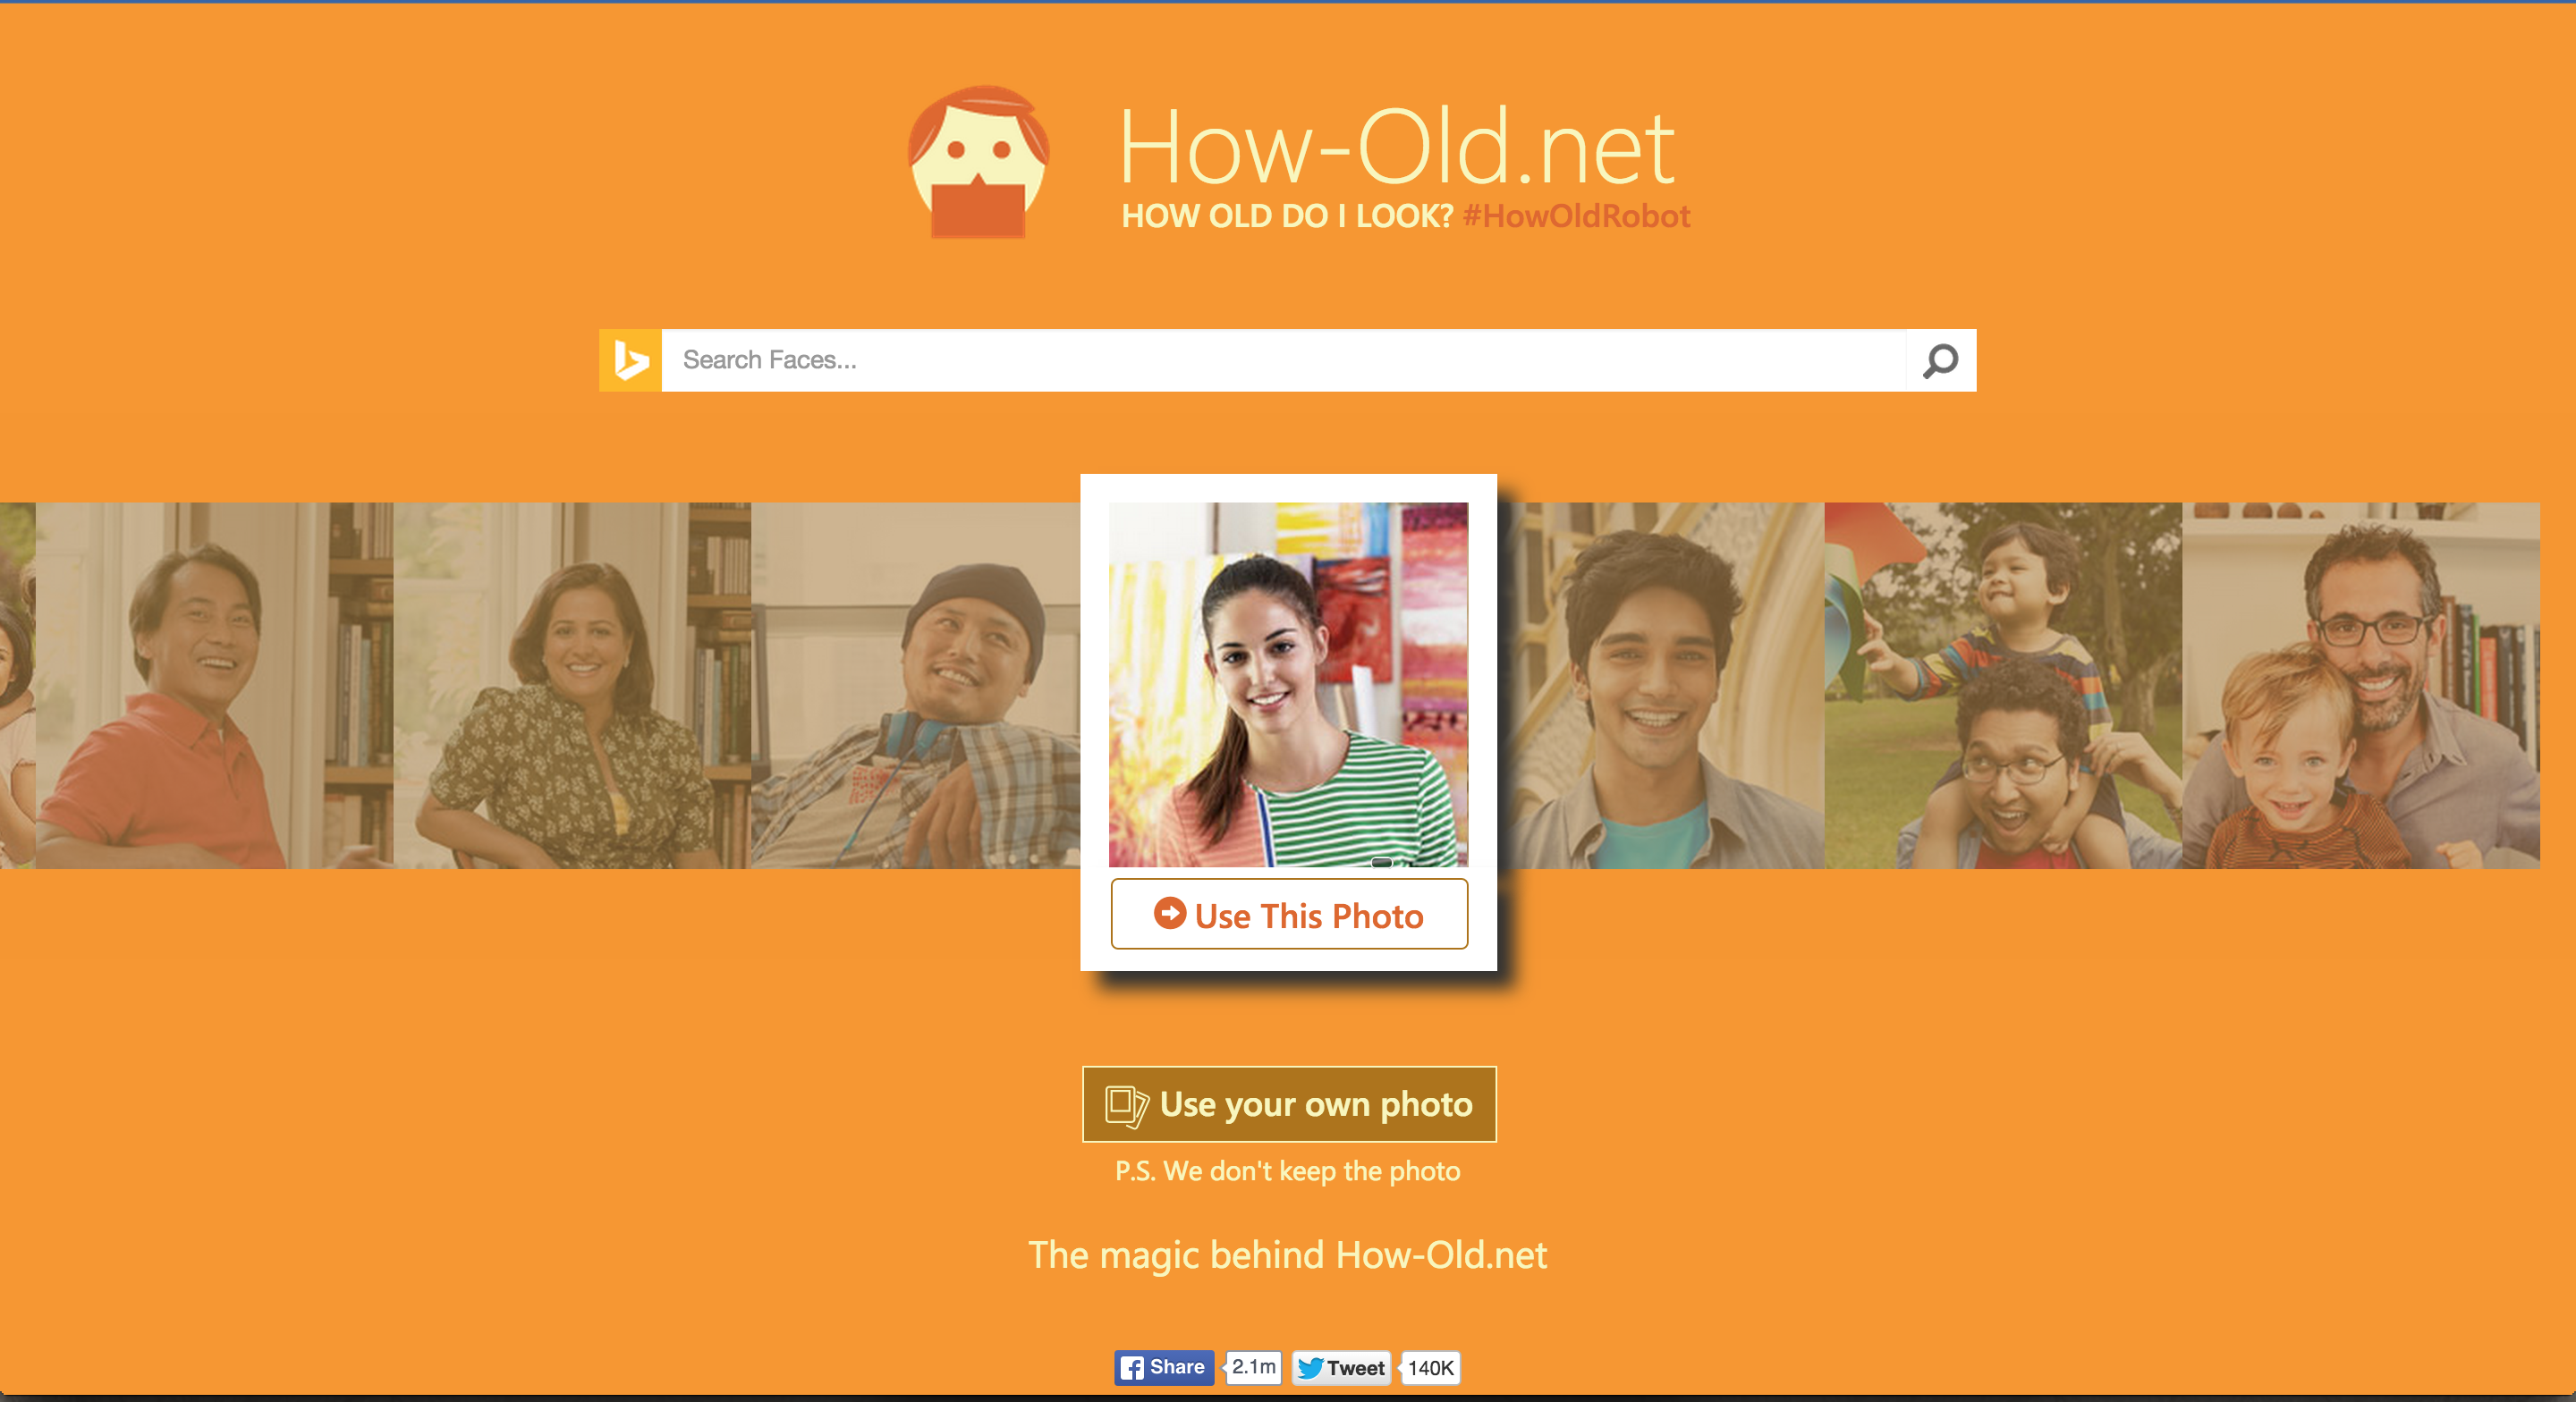
\includegraphics[width=\textwidth]{img/chap5/how_old.png}
\caption{How old from Microsoft\label{Face++API}}
\end{minipage}
\end{figure}
本文的匹配算法经过了一定量用户的检验,反映的效果比较良好,
但在实验中对于用户的分析有一个缺点,是由于用户年龄的不协调性可能导致匹配到的结果效果并不好,但随着图片技术的发展(例如Microsoft的How old,如图5.2所示,可以大致检测出人的年龄),使得我	们可以在之后的工作中,为用户添加上这一特征值,从而进一步提供匹配算法的的准确性,降低这种差异给我们算法带来的不确定性。

而更进一步的由于图片应用的火热和扩展性,可以不断扩充用户,并且不断通过更多的用户提交的信息的特征提取出来,来优化我们的匹配算法,达到更好的效果。


% \section{匹配算法实验}
% \subsection{根据人脸相似度的匹配}
% \subsection{根据具体人脸特征的匹配}
% \subsection{根据具体信息的匹配算法}
% \subsection{机器学习算法}



